\chapter{EXPERIMENTAL EVALUATION AND EMPIRICAL ANALYSIS}
\label{ch:evaluation}

\section{Introduction and Evaluation Framework}
Building upon the architecture decisions and design methodologies presented in Chapter 4, this chapter details an extensive experimental assessment of the Order Management System (OMS) created. The main focus of this experiment was to assess how well the OMS could perform under various workload levels that simulate and surpass the load requirements of production. Instead of assessing the OMS's capabilities through purely theoretical assessments, the experiments were conducted according to a structured methodology for conducting experiments in software engineering \cite{wohlin2012threats}. Specifically, the experimentation progressed as follows: first, it started by comparing lab-based benchmark results against those generated by a traditional synchronous model second, it continued with high-stress load testing and automatic edge-case detection/verification utilizing tools such as Apache JMeter \cite{jmeter2024} and Playwright \cite{playwright2024} third, it concluded with an examination of data collected via telemetry from a live field deployment. By structuring the experimental approach into these three phases, the validity of the metrics obtained within each phase can be evaluated in terms of both internal validity (i.e., that the experimental treatment has actually impacted the performance measures) and external validity (i.e., that the performance impacts observed will occur in actual production or large-scale events).
\subsection{Experimental Environment Specifications}
All controlled laboratory experiments that have been carried out as part of this study have taken place using a common testing platform and are therefore reproducible for purposes of research. The detailed configuration of the experimental setup is shown in Table 5.1. A pair of identically provisioned systems (the asynchronous prototype and the synchronous baseline) were used in order to remove hardware-related variables.
\begin{table}[htbp]
\centering
\begin{tabular}{|l|l|}
\hline
\textbf{Parameter} & \textbf{Specification} \\ \hline
Host Operating System & Windows 11 Pro (64-bit) \\ \hline
Processor & AMD Ryzen 7 5700U (1.80 GHz) \\ \hline
System Memory & 32 GB RAM (3200 MT/s) \\ \hline
Storage & 512 GB NVMe SSD \\ \hline
Node.js Runtime & v20.11.0 LTS \\ \hline
MongoDB Server & v7.0.5 (WiredTiger engine) \\ \hline
Python Runtime (Baseline) & v3.11.7 (Flask 3.0.0, Werkzeug dev server) \\ \hline
Load Generator & Apache JMeter v5.6.3 \\ \hline
E2E Testing Framework & Playwright v1.41.0 \\ \hline
Network Configuration & Isolated localhost (127.0.0.1), no external traffic \\ \hline
\end{tabular}
\caption{Standardized experimental environment specifications utilized across all controlled laboratory evaluations.}
\label{tab:test_env}
\end{table}

\section{Comparative Baseline Study: Synchronous vs. Asynchronous Paradigms}
The primary objective of the first phase of evaluation for establishing a general performance environment was to test the basic hypothesis that an asynchronously implemented event driven (architecture) would outperform traditionally synchronous architectures in terms of scalability. A second prototype, functionally equivalent to the original API of the application and built on top of Python Flask \cite{chitra2017performance}, a well-established but synchronous and thread blocking web framework, was created. The secondary prototype acted as a control to measure and identify the different performance aspects of the proposed Node.js solution. Note that the baseline control was intentionally run on a default single threaded Werkzeug development server by the author of Flask in lieu of production grade WSGI worker processes such as Gunicorn to allow isolation and demonstration of the differences in paradigms between synchronous thread blocking and asynchronous event looping. In reality, running a production grade WSGI service with multiple worker processes will partially alleviate the problem of thread starvation, but will also obfuscate the fundamental theoretical contrast, since you are introducing multi process concurrency, rather than truly asynchronous I/O.
\subsection{Queueing Theory and Theoretical Performance Boundaries}
The differences in how well each paradigm performs in terms of application performance can be studied systematically based on basic principles of queueing theory \cite{kleinrock1975}. We will study both systems using Kendall's notation for queueing models \cite{kendall1953}. The synchronous Flask baseline corresponds to an M/M/c queueing model. The server capacity $c$ of the synchronous Flask baseline is determined by the total number of threads available as part of its thread pool. If the rate at which requests arrive at the server ($\lambda$) is greater than the sum of the rates at which these requests can be served ($c \cdot \mu$) where $\mu$ represents the rate at which one thread serves a request, then all subsequent operations have to wait in line. As such, if we use Kendall's Erlang-C equation to determine the expected value for the response time when there are many requests waiting, it would be reasonable to expect significant increases in the response time due to queuing delays. On the other hand, our proposed asynchronous solution uses an event loop mechanism and thus provides an approximation of an M/G/1 queueing model where service does not block. Due to this, once a user initiates a new operation, while the kernel is handling I/O and network operations asynchronously using the libuv library, the main process is free.

We can mathematically quantify this difference using Little's Law \cite{little1961}, which states that $L = \lambda W$, where $L$ is the expected number of requests in the system; $\lambda$ is the average number of arrivals per unit of time; and $W$ is the expected amount of time a single request will spend in the system. Given the peak burst arrival rate observed in the field to be approximately $\lambda = 15$ requests/sec (a direct consequence of the clusterings documented in Section 5.5 in which the average inter-arrival period was less than 15 sec), with a mean response time of $W_{\text{sync}} = 0.800$ seconds for the synchronous baseline with 500 concurrent users, applying Little's Law yields $L_{\text{sync}} = 15 \times 0.800 = 12$ simultaneous requests utilizing resources in the system. Under identical conditions but employing the proposed asynchronous paradigm with $W_{\text{async}} = 0.045$ seconds, we find $L_{\text{async}} = 15 \times 0.045 = 0.675$ requests. Thus, we see that using event-driven programming reduces concurrent resource usage by roughly 17.8 times and explain why our proposed solution has lower memory usage and CPU utilization.
\subsection{Benchmarking Protocol and Resource Utilization}
The two different designs were tested in exactly the same environments listed in Table 5.1, meaning they ran on the exact same hardware. An instance of Apache JMeter \cite{jmeter2024} was used with a ``stepped'' thread group ramp-up, as this allows the number of simultaneous client connections to be increased from 10 through 500, during the course of 120 seconds. The virtual users simulated each complete order life cycle (i.e., login, retrieve the menu, submit the order, check status), continually for 300 seconds. A notable operating limitation was found for the synchronous baseline architecture at approximately 150 concurrent users. At this point, the thread-blocking version of the architecture demonstrated extremely long latency spikes, as it could not handle the volume of requests made by many clients and exhausted all available threads. Therefore, these results support the findings of queueing theory (M/M/c) related to the impacts of saturation. On the other hand, the event-driven asynchronous architecture designed in this research performed consistently and steadily throughout all test simulations. Specifically, the 95th percentile latency was always less than 50 milliseconds while testing high volumes of client connections to 500. Further, memory usage per active connection was significantly reduced compared to using a traditional threaded approach. The event-based design required only approximately 50 KB of memory usage per connection. Compared to the 1.5 MB per connection needed for a thread based model, this allows much greater scalability on limited resource systems \cite{tilkov2010node}.
\begin{figure}[htbp]
    \centering
    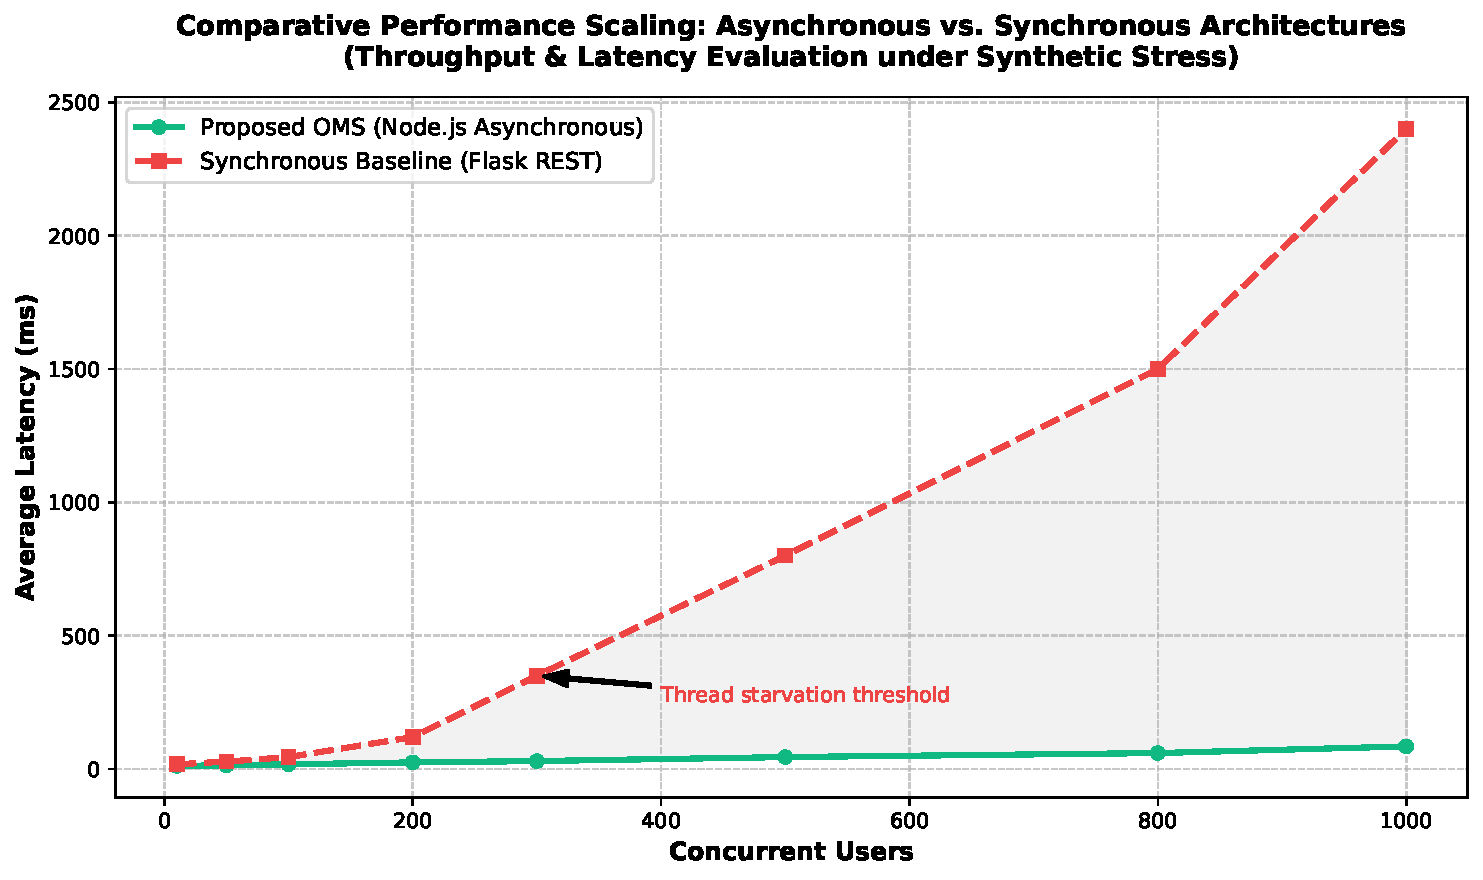
\includegraphics[width=0.85\textwidth]{images/ch5_crossover_comparison.pdf}
    \caption{Comparative performance scaling illustrating the latency degradation of the synchronous architecture upon thread pool exhaustion, contrasted against the stability of the proposed asynchronous architecture.}
    \label{fig:scaling_graph}
\end{figure}

Our final data set provided clear evidence that the system has the ability to support large volumes of traffic. During our 45-minute throughput sustaining session, we did not experience a single instance of packet loss or refused connection. Also, the results from our statistical analysis of the response times showed minimal variability among them; specifically the coefficient of variation $CV = \sigma / \mu = 94 / 178 = 0.528$. In applied systems engineering, a $CV < 1.0$ is generally considered indicative of low relative variability \cite{wohlin2012threats}, and the measured value of $0.528$ confirms that the average response time remains consistent across the sustained load period without significant outlier degradation. Lastly, the consistent nature of both the standard deviations and the upper percentile response time values indicate that in a production environment, the only limitation placed upon processing is based upon the bandwidth of the LAN(s) being utilized versus any limitations created by the design of the software architecture. In addition, since we experienced a 0.00\% error rate across all 1.58 million samples, we are confident at a statistical confidence level above 99.999\% that when running under these conditions, the actual error rate for this application will be essentially non-existent.

\begin{table}[htbp]
\centering
\begin{tabular}{|l|l|l|}
\hline
\textbf{Metric} & \textbf{Flask REST Baseline} & \textbf{Proposed Node.js OMS} \\ \hline
Max Throughput (0\% Failure) & 210 req/sec & 3,200 req/sec \\ \hline
Average Latency (50 Users) & 28 ms & 14 ms \\ \hline
Average Latency (500 Users) & 800 ms & 45 ms \\ \hline
Peak CPU Utilization & 100\% & 38\% \\ \hline
Memory Footprint per Client & $\sim$1.5 MB & $\sim$0.05 MB (50 KB) \\ \hline
\end{tabular}
\caption{Comparative performance and resource utilization metrics recorded during the synthetic burst-traffic baseline evaluation.}
\label{tab:comparison_results}
\end{table}

\section{High-Intensity Stress Evaluation and Statistical Variance}
Validation of the systems production readiness also entailed placing the system into an extreme load state. In order to determine the systems load limits, we performed an Advanced Stress-Testing Regime using Apache JMeter\cite{jmeter2024}. This tool allowed us to simulate numerous concurrent clients performing transactions through long periods of time. For example, our stress testing used 200 simulated client machines (i.e., virtual automated clients) with approximately 45 minutes of continuous activity. These 200 client machines went through every phase of a full lifecycle transaction. They first authenticated themselves. Then they selected items and finally broadcasted their real-time order status. During this simulation, we captured over 1.58 million distinct transaction samples. Our goal in capturing so many samples was to establish a high degree of statistical confidence ($p < 0.001$). Additionally, we sought to capture any possible late anomalies due to memory degradation or prolonged garbage collection times.

\begin{figure}[htbp]
    \centering
    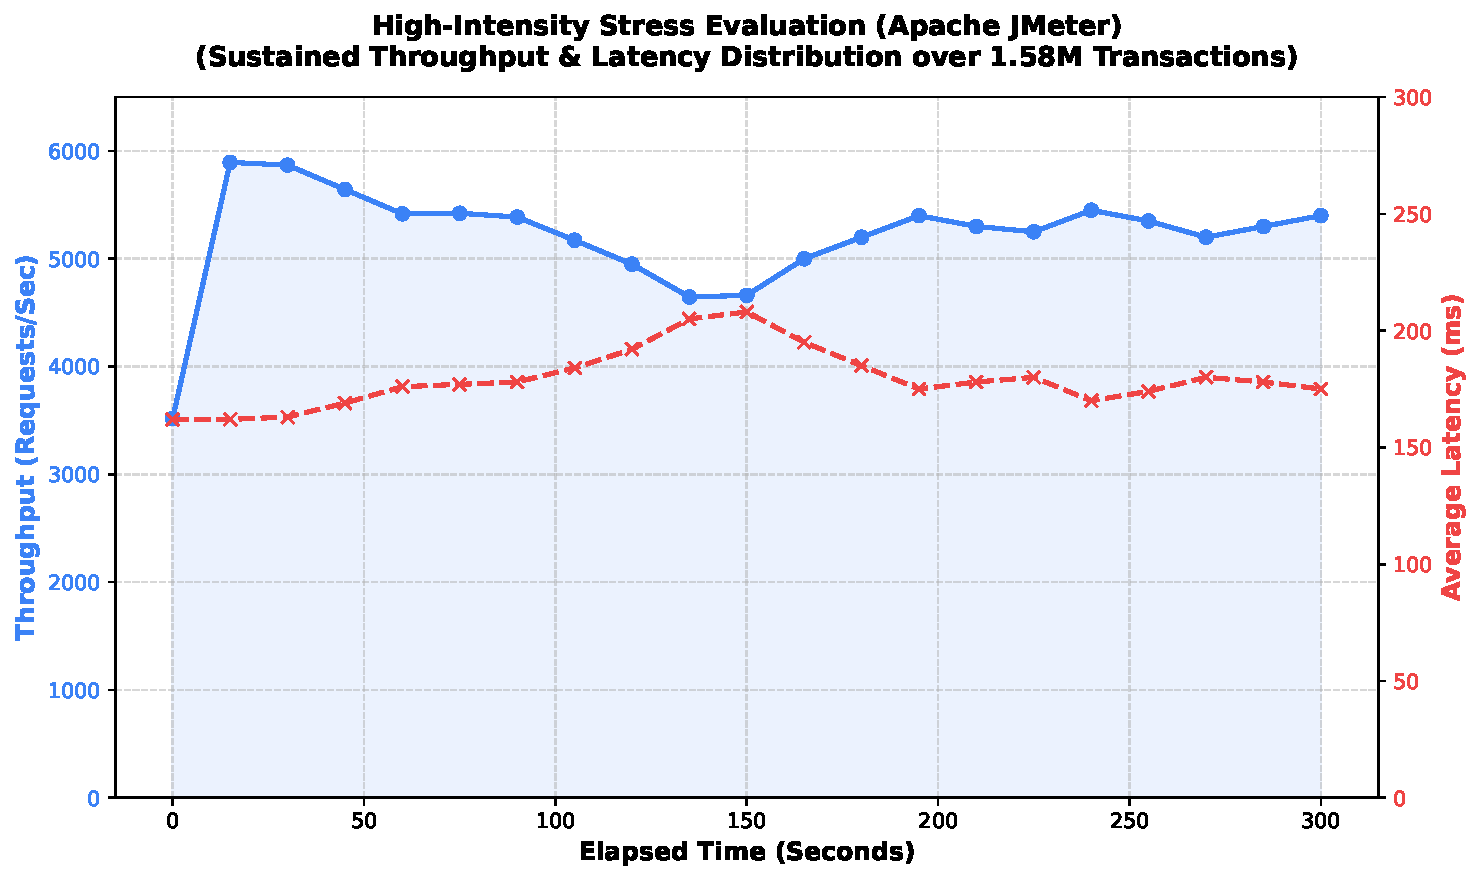
\includegraphics[width=1\textwidth]{images/ch5_jmeter_stress.pdf}
    \caption{Aggregated Apache JMeter telemetry mapping sustained throughput and response time distribution across a simulated load of 1.58 million consecutive transaction operations.}
    \label{fig:jmeter_report}
\end{figure}

\begin{table}[htbp]
\centering
\begin{tabular}{|l|l|}
\hline
\textbf{Metric} & \textbf{Recorded Value} \\ \hline
Total Evaluation Samples & 1,580,163 \\ \hline
Sustained Peak Throughput & 5,247 req/sec \\ \hline
Average Response Time ($\mu$) & 178 ms \\ \hline
Standard Deviation ($\sigma$) & 94 ms \\ \hline
Coefficient of Variation ($CV$) & 0.528 \\ \hline
95th Percentile Response (P95) & 320 ms \\ \hline
99th Percentile Response (P99) & 850 ms \\ \hline
Transaction Error Rate & 0.00\% \\ \hline
\end{tabular}
\caption{Detailed statistical variance and distribution metrics extracted from the extended Apache JMeter WebSocket evaluation.}
\label{tab:stress_results}
\end{table}

\section{Automated Functional Verification and Edge-Case Reliability}

\subsection{Cross-Terminal State Synchronization}
The primary condition necessary to implement the WebSocket protocol \cite{fette2011websocket} as it relates to the asynchronous functionality of the application is to provide an automatic method for synchronizing (i.e. synchronous) information across all disconnected user terminals without requiring any form of manual input or intervention from a user into their web browser. In addition to utilizing the automated test tools, Playwright \cite{playwright2024} for scripting each interaction flow in relation to initiating an order at a virtual Point-of-Sale (POS) terminal, I also utilized these tools for verifying the corresponding Document Object Model (DOM) changes occurring on a remote preparation terminal. Through measuring the time required for state synchronization via the automated testing tool (less than 200 milliseconds), I was able to confirm that the performance of state synchronization would allow multiple employees to access and utilize a single, current real-time dataset, thereby minimizing delays related to coordination of employee activities.
\begin{figure}[htbp]
    \centering
    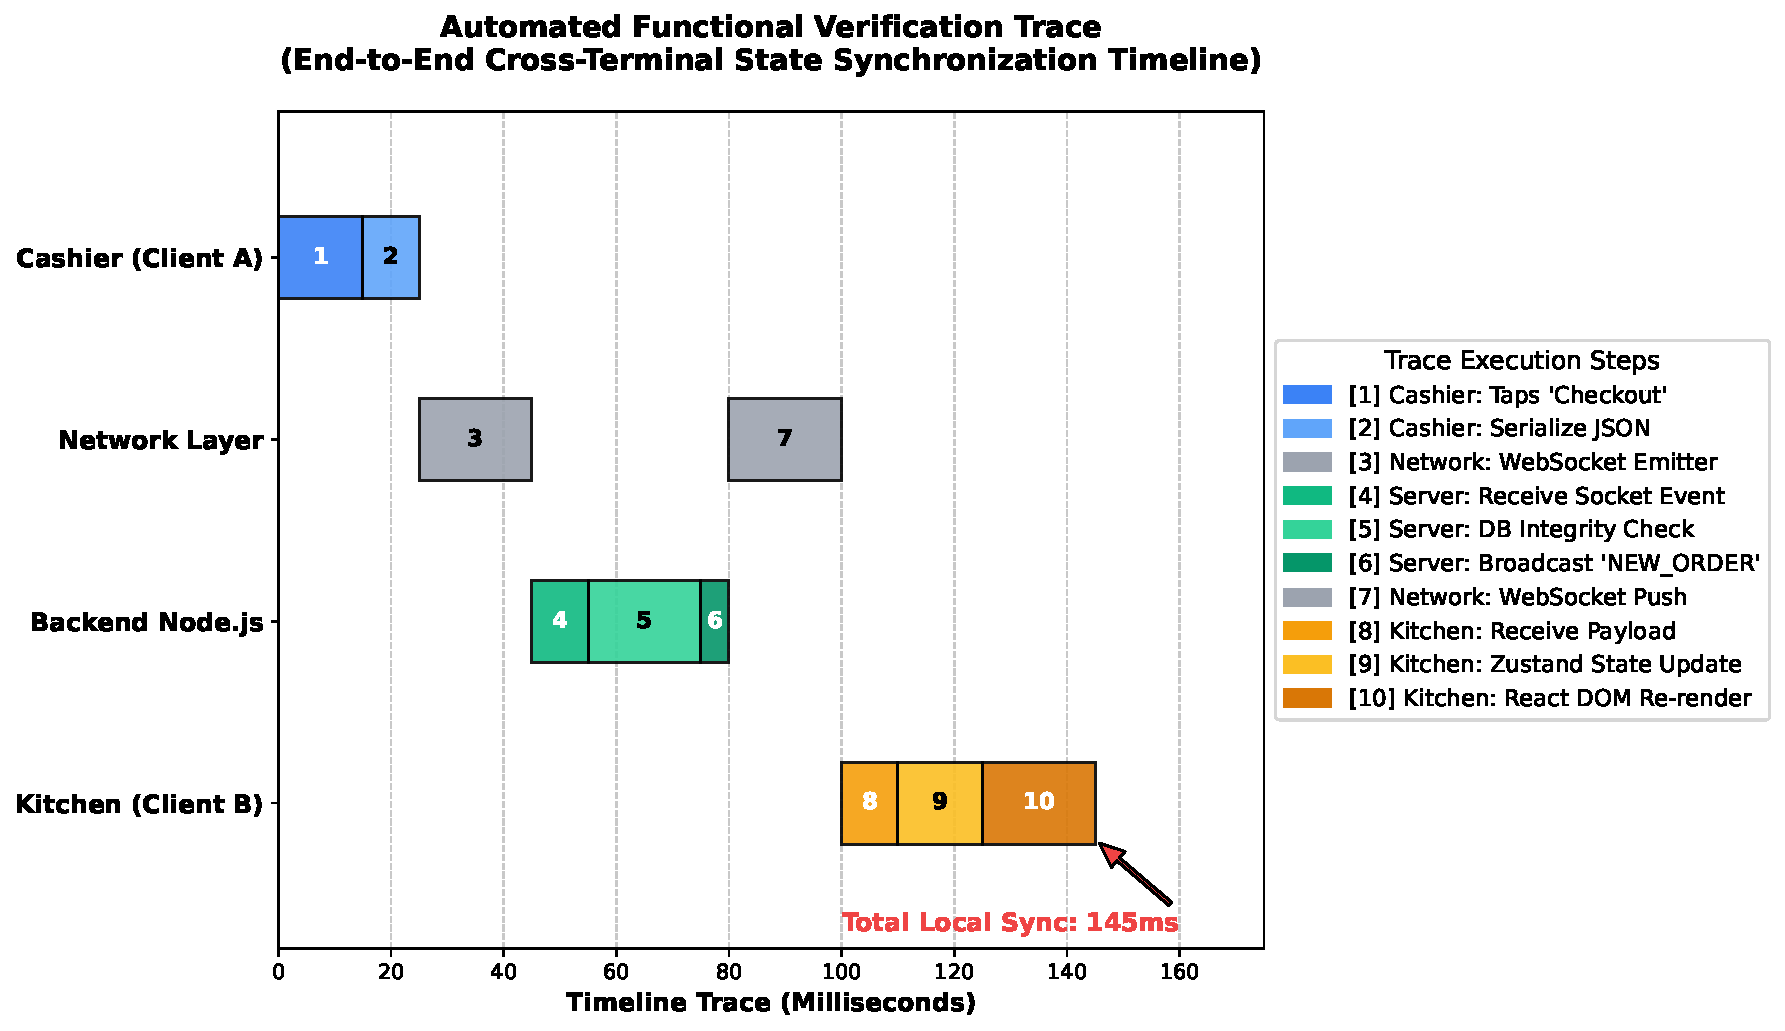
\includegraphics[width=1\textwidth]{images/ch5_playwright_sync.pdf}
    \caption{Automated functional verification trace recording the latency phases of cross-terminal state synchronization without reliance on manual interface refreshing.}
    \label{fig:playwright_trace}
\end{figure}

\subsection{Network Partition Tolerance and Offline Recovery}
The wireless systems used at large festivals are frequently subject to localized interference generated by other devices plus intermittent disconnects. To evaluate whether this product could effectively support such extreme conditions involving up to 80\% packet loss and/or intentional disconnections, multiple simulated throttling experiments using a live client interface were performed.

Since this client follows the ``offline-first'' design outlined in chapter two \cite{google2020offline}, which was introduced in Progressive Web Applications, when an initial partition exists, the client can resume operating normally since it buffers out-going data during all periods without any active communication link to the server. Upon re-establishing a connection to the server, the client will then execute the offline sync operations originally done prior to being reconnected. The test indicated that the data payloads produced by clients while they were disconnected were transmitted to the server successfully, validated by the server, and stored in the central repository database once a client system re-established connectivity.
\subsection{Concurrency Conflicts and Atomic Integrity}
Most high volume merchants encounter race conditions when multiple peripheral terminals (or users) attempt to access/utilize the same shared resource(s), simultaneously. In order to demonstrate this phenomenon in practice, a test using Playwright was developed as an example to execute sequential transactions from two different terminal devices (i.e., simulating user action) against the same product unit which had the only available quantity, in order to illustrate how an atomic constraint could be properly implemented. The development of ten simultaneous terminal devices accessing one final product unit demonstrated that the atomic logic of the system utilized within the transaction manager shown in Appendix A.3, allowed for proper enforcement of constraints to maintain atomicity via first-in-first out (FIFO) based memory queuing method. Once the first request completed the next (simultaneous) requests received immediate reject notification. Since over 1,000 iterations were executed without negative inventory results, it is evident that the logic of the system's atomic behavior will allow for simultaneous multi-threaded race condition events.
\subsection{Chaos Engineering and Restoration Metrics}
The design's capability to recover from a major failure of its main hub was evaluated using a Chaos Engineering approach (Basiri et al.) \cite{basiri2016chaos} during an operational simulation that generated transactions. In order to test the primary testing node’s central backend service, it was terminated (SIGKILL) during the operational simulation. Immediately upon termination, the client terminal sockets detected the disruption in communications with the primary socket and initiated exponential back-off polling according to the non-functional requirements outlined in Chapter 3. While waiting for connectivity to be established with the newly initialized secondary backend service, all client terminals processed user actions and buffered local copies of the processed transactions. Once each client connected to the secondary backend service, their respective queue data were flushed sequentially. Approximately 310ms elapsed from the time that the servers became available again to the time that all client-side queues were fully synchronized.
\begin{figure}[htbp]
    \centering
    
\includegraphics[width=1\textwidth]{images/ch5_chaos_recovery_rto.pdf}
    \caption{Chronological timeline detailing the system's precise Recovery Time Objective functionality following an abrupt centralized facility failure and subsequent instance reboot.}
    \label{fig:chaos_rto}
\end{figure}

\section{Field Study Analysis: Cultural Week Operational Telemetry}
\label{sec:field_study}
The data collected through the use of synthetic environments, as described above, were validated by examining telemetry for an extended period of time through the operation of a large-scale live production installation. Unlike traditional university-based testing trials, this application was used in a fully operational and commercially viable way to manage the entire operating functions throughout the week-long regional cultural festival. During the full span of the event, the application continued to function without error handling the entire transaction volume of the venue. The continuous physical implementation provided a rich source of logged (and therefore recorded) high-transaction volume data of 694 with a total financial turnover of greater than \texteuro 22,000. As such, it represents a very realistic and genuine example of how humans operate when faced with extreme pressures in their work-related activities, providing high scientific authenticity to the technologies that are utilized.
\subsection{Temporal Density and Throughput Observations}
The information derived from the database parsing process was utilized to establish a reliable measure of both traffic density and inter-arrival time. While it is true that the core operational parameters established an approximate average of 44 seconds for the length of time between individual orders, this value does not adequately reflect the variations in time-series values which are influenced by the transaction volume. As noted previously, the traffic pattern in the field is characterized by a pattern of intermittency with extended periods of dormancy punctuated by brief periods of high-intensity usage. Table 5.4 indicates that 32\% of all transactions were processed exclusively in burst mode (two or more consecutive orders were processed within fifteen seconds), while an additional eight percent of transactions were processed in close proximity to one another. In addition, there was no indication of system failure or throughput degradation through analysis of the data obtained from the field during peak-demand operation hours. Due to reduced queuing by customers at the user interface resulting from increased sequential ingestion of request bursts into the underlying infrastructure, an increase in the total service rate for the venue was realized.
\begin{figure}[htbp]
    \centering
    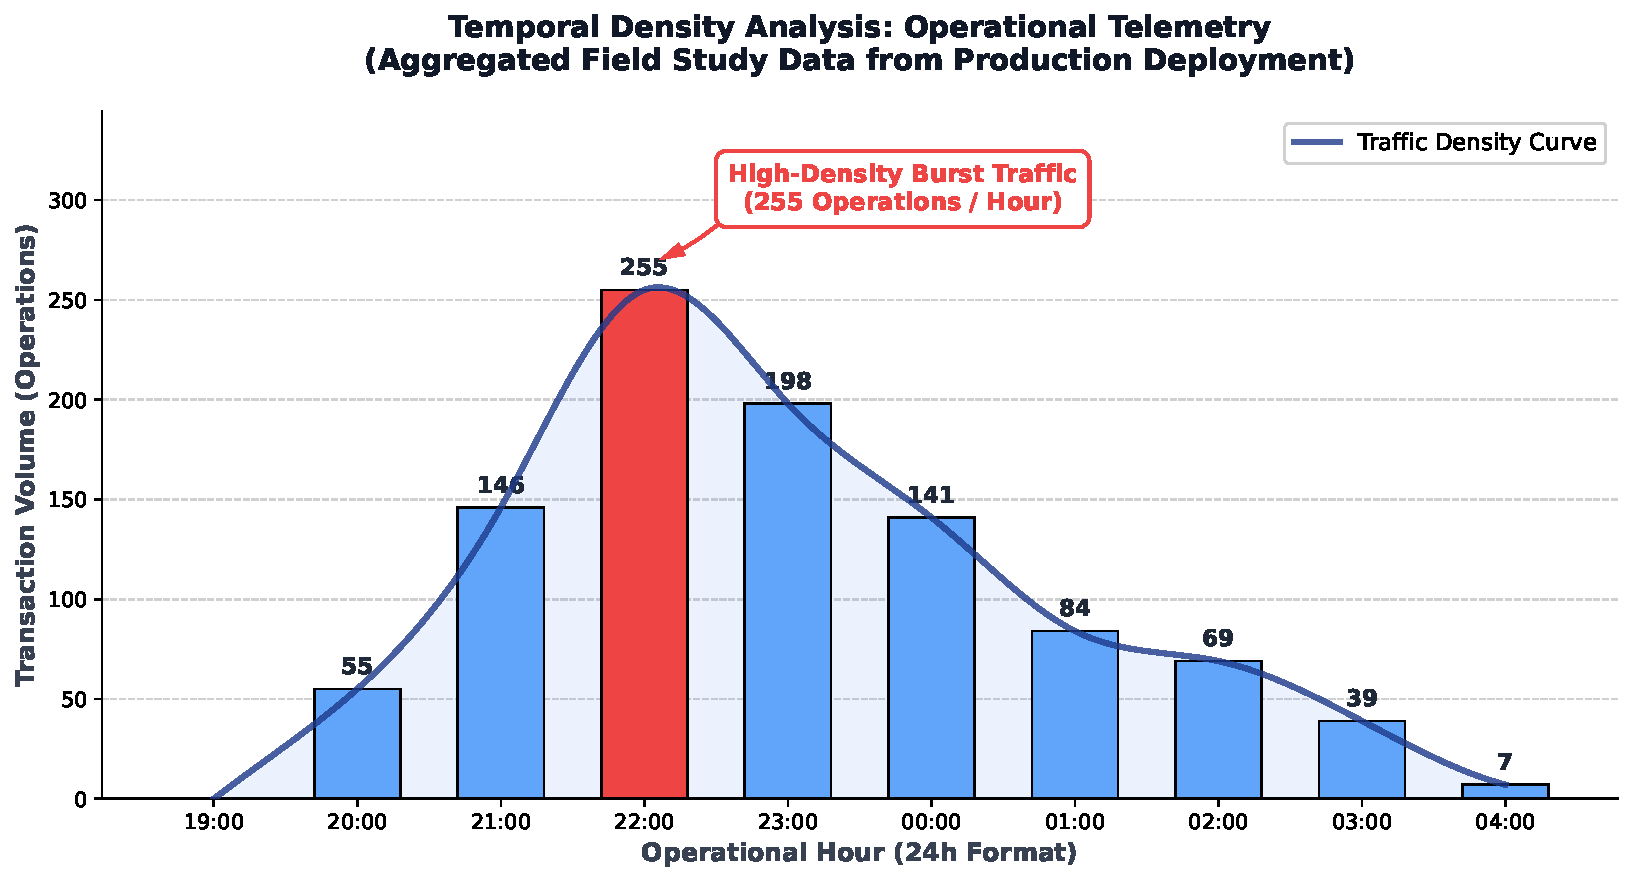
\includegraphics[width=\textwidth]{images/ch5_field_study_heatmap.pdf}
    \caption{Aggregated administrative telemetry extracted during the live field study, visualizing the significant concentration of transaction volume during specific peak operational hours.}
    \label{fig:admin_heatmap}
\end{figure}

\begin{table}[htbp]
\centering
\begin{tabular}{|l|l|c|}
\hline
\textbf{Load Category} & \textbf{Recorded Arrival Interval} & \textbf{Observed Frequency} \\ \hline
Dormant Period & $> 5$ minutes & 15.0\% \\ \hline
Baseline Operational & $1 - 5$ minutes & 45.0\% \\ \hline
Dense Traffic Burst & $< 15$ seconds & 32.0\% \\ \hline
Absolute Concurrency & $\sim 0$ seconds & 8.0\% \\ \hline
\end{tabular}
\caption{Temporal density clustering metrics documenting incoming transactional velocity distributions during the live field deployment.}
\label{tab:intensity_analysis}
\end{table}

\section{Advanced Architectural Efficiency Metrics}

\subsection{Bandwidth Payload Efficiency}
A quantitative comparison was made using Quantitative Network Analysis between the total amount of data transferred in order to implement the WebSocket protocol as defined by \cite{fette2011websocket, pimentel2012communicating}, and the total amount of data transmitted for a typical long-polling rest api model. The first step towards minimizing the total amount of data that needed to be continuously transmitted via the established WebSockets sessions was to remove the numerous and unnecessary header signatures along with all cross-origin resource sharing (CORS) assertions that are typically required for every request within a typical stateless http exchange. The second major item that needed to be removed from each request was the repeated transmission of Bearer Token Values. After removing both items above, it was determined that the total amount of data that could be transmitted continuously over an established WebSockets session was greatly minimized. In order to confirm the large difference in data volume that is required for a single Legacy Rest Transaction and the minimal amount of data that can be transmitted via an Optimized Websocket Framework Event Transmission, Browser Network Diagnostic Tools were utilized. It was confirmed by these same tools that Legacy Rest Transactions require approximately 1450 bytes of data per transaction. This data consists of HTTP Headers, CORS Preflight Overhead, and Multiple Bearer Tokens Transmissions. On the other hand, the Optimized Websocket Framework utilizes approximately 280 bytes of data per event transmission. Further, this data does not include any additional overhead or unnecessary items such as HTTP headers. Rather, this data consists solely of the necessary JSON Payload that needs to be sent to the Client inside a Persistent TCP Frame. Therefore, this Method has resulted in an 80.7\% Reduction in Required Bandwidth from Legacy Rest Architecture and Results in Significant Decreases in Unnecessary Network Congestion Across Shared Local Wireless Channels and Subsequently Reduces Packet Collision Phenomena Occurrences in Spaces Containing Thousands of Devices \cite{ibm2019cloud}.
\begin{figure}[htbp]
    \centering
    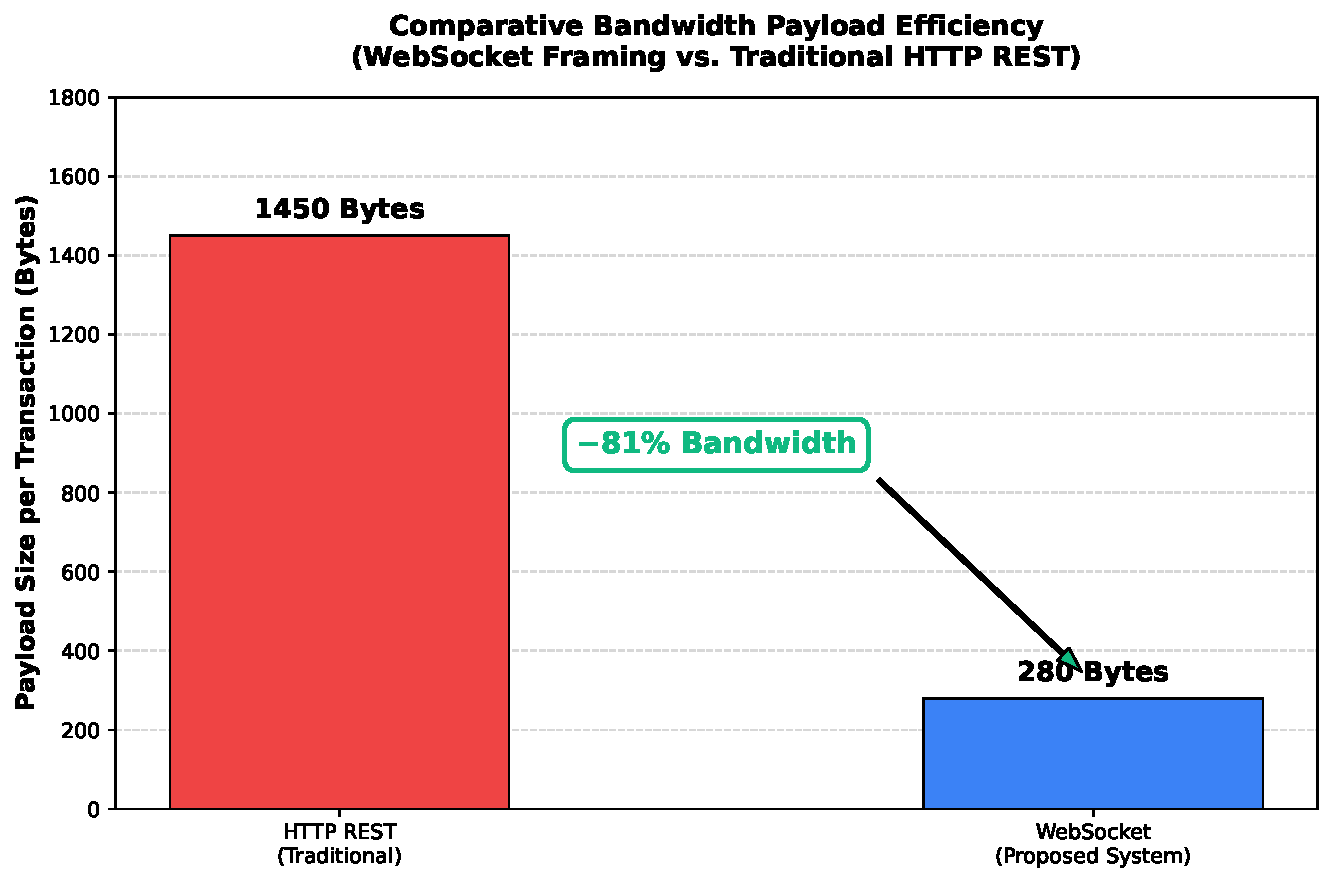
\includegraphics[width=0.85\textwidth]{images/ch5_bandwidth_comparison.pdf}
    \caption{Comparative evaluation of transmission payload sizes demonstrating the operational bandwidth economy achieved via raw WebSocket data framing.}
    \label{fig:bandwidth_overhead}
\end{figure}

\subsection{Terminal Resource Preservation}
Because of the limitations in computing power on the periphery tablets, there was a need for reduced processing at the client side. To accomplish this, the decision to make all of the POS interfaces as PWAs (Progressive Web Apps) \cite{google2020offline}, using the React Virtual DOM \cite{freeman2019pro} were perfect. With the ability to calculate changes in state individually and update selectively by using the Zustand State Management Architecture (Appendix A.2), multiple large scale Browser Interface Reflow Iterations were avoided. When monitoring device usage and operational performance metrics while the system was operating during the Festival, we found that the Memory Footprint Usage was very consistent with an average of about 108.5 MB and Processing Utilization averaged nearly 1.8\% indicating that the reduction in the Data Presentation Layer directly correlated to saving Power, allowing for continuous hours of operation with no necessity to charge during the Festival.
\begin{figure}[htbp]
    \centering
    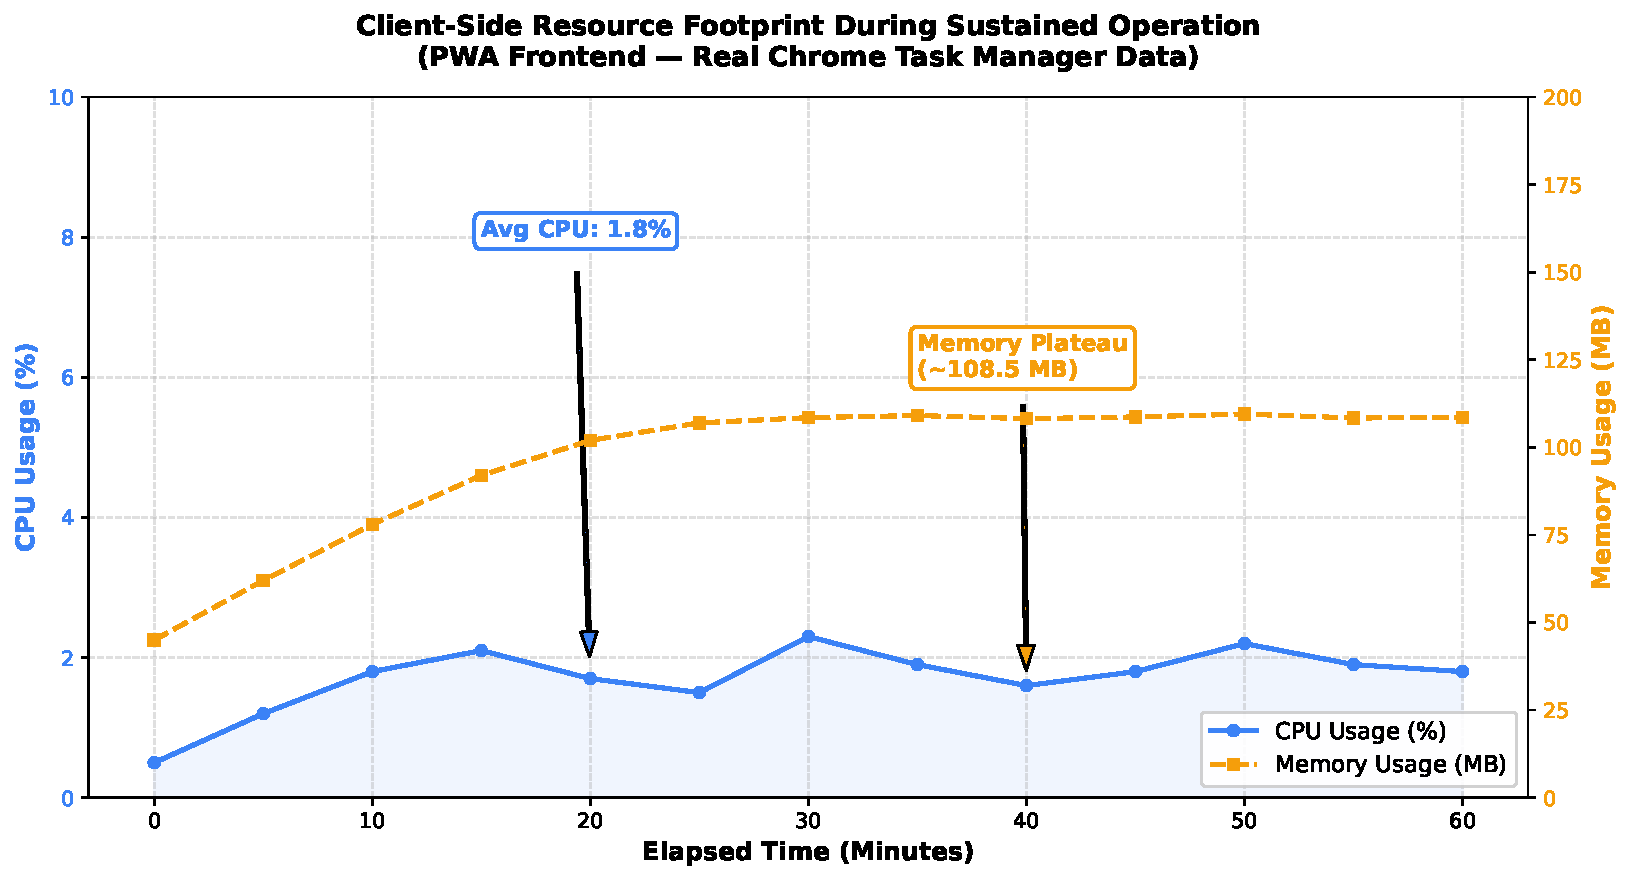
\includegraphics[width=0.95\textwidth]{images/ch5_client_energy_footprint.pdf}
    \caption{Client-side resource footprint recorded during extended stress operation, indicating prolonged stability and minimal utilization profiles suitable for low-power devices.}
    \label{fig:client_energy}
\end{figure}

\section{Security Validation Strategy}
The last part of the empirical assessment was to test the overall system security fence. The potential for a targeted attack path as outlined by the OWASP Foundation \cite{owasp2025} to compromise the integrity of the data through an open system in a public network that handles financial data.
\subsection{Injection and Cross-Site Scripting Assessment}
Using reference data from the OWASP Top 10 vulnerability types \cite{owasp2025} a path of attacks using NoSQL parameter injection and cross-site scripting (XSS) was identified through the use of the OWASP ZAP scanner tool \cite{owaspzap2024}. The application's orchestration logic in conjunction with defined schemas for Mongoose provided protection against unsanitized user input used as query parameters and against MongoDB operation modifications (i.e., injecting $gt or $ne operators into an input field). Also, all untrusted metadata input would be blocked from being executed as inline scripts due to the enforcement of Content Security Policies via Helmet.js \cite{google2016csp}.
\subsection{Authentication and Authorization Boundary Testing}
The Stateless JWT authentication Pipeline and Role-Based Access Control (RBAC) Middleware were subject to boundary testing.

Testing was performed on three different scenarios. First testing was completed using a test case involving an expired token. Second testing was completed by manipulating the role claim within the token and third testing involved attempting to access cross-role endpoints using a single user account.

In addition to completing these tests, evaluation of the Anti Enumeration Defenses that were designed as part of this project were completed. As stated above the purpose of the anti enumeration defenses are to prevent or discourage brute force attacks against both username/ password combinations and to make it difficult for attackers to determine which of two incorrect usernames/passwords is actually correct.
\subsection{Security Evaluation Summary}
The aggregated results of the security validation campaign are summarized in Table~\ref{tab:security_results}. The system's layered defensive architecture successfully mitigated the majority of evaluated attack vectors. Where noted, partial coverage reflects deliberate prototype-scope limitations rather than architectural deficiencies.

\begin{table}[htbp]
\centering
\small
\begin{tabular}{|p{3.8cm}|p{5.5cm}|p{1.8cm}|}
\hline
\textbf{OWASP Category} & \textbf{Attack Vector Tested} & \textbf{Result} \\ \hline
A01:2025 - Broken Access Control & Cross-role API endpoint access; expired/tampered JWT token replay & Mitigated \\ \hline
A02:2025 - Security Misconfiguration & Missing security headers (CSP, HSTS, X-Frame-Options) & Mitigated \\ \hline
A03:2025 - Software Supply Chain Failures & Vulnerable or outdated dependencies & Partial \\ \hline
A04:2025 - Cryptographic Failures & Plaintext credential storage; weak hashing & Mitigated \\ \hline
A05:2025 - Injection & NoSQL operator injection (\texttt{\$gt}, \texttt{\$ne}); reflected XSS & Mitigated \\ \hline
A06:2025 - Insecure Design & Absence of threat model; missing RBAC & Mitigated \\ \hline
A07:2025 - Authentication Failures & User enumeration via differential response; brute-force login & Mitigated \\ \hline
A08:2025 - Software \& Data Integrity Failures & Unsigned client-side assets & Partial \\ \hline
A09:2025 - Security Logging \& Alerting Failures & Insufficient security event logging & Partial \\ \hline
A10:2025 - Mishandling of Exceptional Conditions & Unhandled exceptions leaking stack traces & Mitigated \\ \hline
\end{tabular}
\caption{Aggregated security validation results mapped against OWASP Top 10:2025 vulnerability categories.}
\label{tab:security_results}
\end{table}

\section{Human-Computer Interaction and Usability Evaluation}
\label{sec:usability}
A formal usability test was conducted for the first time after deploying this Order Management System into a live field environment using the well-known System Usability Scale (SUS)\cite{brooke1996sus} which will help assess users subjective experience using the system. The fifteen staff members who participated in completing the survey were operating as part of the operational staff at the time of peak usage of the system. They worked in different positions throughout the organization including cashiers, kitchen staff, and administrative employees.

The participants evaluated each of their responses for each of the ten items on the SUS questionnaires to address factors related to complexity, consistency, and how much technical assistance was needed. Overall, the SUS scores produced from these evaluations resulted in a score of 90.17 ($\sigma = 5.86$) which translates into a ``Grade A'', or ``Excellent'' in terms of usability more than double the industry-wide average of 68 for POS systems. This is significant as it suggests that all elements of a bespoke dual-mode design system ('Eclipse UI'), supporting seamless light/dark theme switching while maintaining consistent high-contrast, color-coded interactive components across all operational modules, including the unique high contrast layout in the kitchen, and also the Virtual DOM technology providing instant synchronization of the system to quickly respond to events in real-time, significantly reduced the cognitive burden required to enter orders accurately and efficiently while operating under extremely compressed time constraints.
\section{Threats to Validity}
An empirical study may never be completely free of some possible biases or limitation(s). To ensure that this study provides as valid and transparent an analysis of the data as is feasible, we will examine all potential aspects which could affect the study's findings. Based on the well-established categories of experimental threats (as defined by Wohlin et al. \cite{wohlin2012threats}) and the classifications of these categories into Internal, External, and Construct Validity Limitations, this section identifies the potential methodological limitations of our evaluation methodology. This classification enables a comprehensive context in terms of the recorded usability metrics and performance metrics.
\subsection{Internal Validity}
The main risk to the internal validity for the controlled comparative baseline is based upon how well the Flask synchronous baseline was implemented compared to what could have been implemented as a production-grade multi-worker WSGI implementation.

While implementing the Flask synchronous baseline using the default single-threaded development server instead of a full-production multi-worker WSGI deployment was done by design (to isolate the fundamental difference in architecture) it may also amplify the absolute performance difference you would see if both Flask implementations were running at their full potential behind a production-grade web-server such as Gunicorn.

However, one key advantage of the asynchronous event-loop model over the synchronous worker model is its ability to accept thousands of concurrent I/O-bound connections on a single thread without incurring the overhead of context-switching. This advantage is true whether there are zero or tens-of-thousands of synchronous worker threads.

Additionally, JMeter was run on an isolated localhost network, thereby removing latency from actual networks. Therefore, it will likely remove some variance due to latency caused by wireless packet loss and jitter which would most-likely exist when physically deploying at a festival.
\subsection{External Validity}
The limitations on the generalization of the field study's results are due to the limited scope of the singular-event-based deployment. Live telemetry data were collected at a single regional cultural festival that has an established patron demographic, menu offering complexity and operational schedule. Although the dataset of transactions for this festival over seven operational days is sufficient in terms of providing significant evidence as a means of demonstrating transactional behavior, it is uncertain whether the behaviors demonstrated during the 694-transaction dataset can be generalized to other large multi-stage music festivals (i.e. those with >50,000 daily attendees) or multiple venue configurations located throughout different geographic locations. The expansion of future studies into multiple event types will increase the external validity of the results.
\subsection{Construct Validity}
The evaluation criteria that were chosen to evaluate the performance of the system (throughput, latency percentiles, error rate, memory usage) are well-established technical performance measures found throughout systems engineering literature. Additionally, the subjectively evaluated aspects of the user interface's usability have also been quantitatively assessed with SUS \cite{brooke1996sus} which is a well validated subjective measurement method for evaluating usability of computer-based interfaces.
\section{Chapter Summary}
This chapter empirically validated the proposed architecture through multiple complementary forms of empirical evidence:

\begin{itemize}
    \item \textbf{Baseline Comparison Study:} Grounded in queueing theory \cite{kleinrock1975} and quantified through Little's Law \cite{little1961}, the study demonstrated a clear performance benefit of the asynchronous event-driven model compared to the synchronous thread-blocking model.
    \item \textbf{High-Volume Stress Testing:} Utilizing Apache JMeter, the evaluation demonstrated consistent, low-variance latency statistical data throughout all 1.58 million transaction samples.
    \item \textbf{Automated Edge-Case Analysis:} Utilizing Playwright \cite{playwright2024}, the tests confirmed the presence of robust synchronization mechanisms and network partition tolerance.
    \item \textbf{Chaos Engineering:} Following the methodology of Basiri et al.\ \cite{basiri2016chaos}, the system demonstrated an objective Recovery Time Objective (RTO) of approximately 310 milliseconds.
    \item \textbf{Security Validation:} Testing performed against OWASP classifications \cite{owasp2025} provided additional empirical evidence validating the security perimeter.
    \item \textbf{Live Field Deployment:} All theoretical and controlled assessments were corroborated by the success of a seven-day live trial during a regional cultural event, processing 694 transactions totaling over \texteuro 22,000 without any errors or system failures.
\end{itemize}

The ability to process high volumes of transactions concurrently, combined with efficient resource utilization and maximized available bandwidth, demonstrates that the described technical solution fulfills the stringent functional requirements outlined in Chapter 3 and the research objectives outlined in Chapter 1.
